\chapter{Wst�p}
Sprawozdanie zosta�o przygotowane w ramach zaj�� z przedmiotu \emph{Sterowanie i symulacja robot�w} w semestrze zimowym roku 2021. Cz�� laboratoryjna zosta�a zrealizowana podczas zaj�� w dniu 19.10.2021. G��wny przedmiot rozwa�a� podczas projektu oraz laboratorium stanowi�a analiza dok�adno�ci przemieszczania si� robota mobilnego podczas wzgl�dnego sterowania pozycyjnego. W pierwszym przypadku robot porusza� si� na podstawie wy��cznie zadawanych pr�dko�ci, a w drugim wariancie wykorzystywa� dane z odometrii. Programy zaimplementowane podczas prac nad projektem zosta�y r�wnie� uruchomione na rzeczywistym robocie \emph{Tiago} firmy PAL w Laboratorium Robotyki na Wydziale EiTI.


\begin{figure}[!htb]
    \centering
    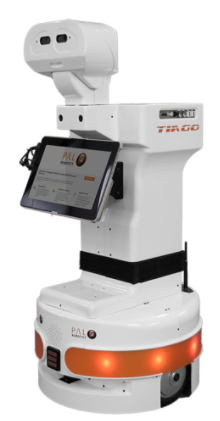
\includegraphics[scale=1]{Projekt_1/plots/tiago}
    \caption{Robot \emph{Tiago} (\emph{Rico})}
		\label{fig:sampleFig}
\end{figure}